\chapter{The Unstructured Heart as a Binary Cube} 
After a MRI scan of the heart, the resulting data are stored as a point cloud, which is a huge collection of unstructured points, that typically needs advanced mesh generation techniques that consists of triangulations of the stored point cloud to form an accurate 3-D model of the human heart, that more specifically, is a large collection tetrahedras. The goal of my implementation is to generate a uniformly structured mesh, using the unstructured data as a basis for checking if a generated point is inside or outside the unstructured heart geometry. The resulting structured mesh will consist of points both inside and outside the heart, but will later be numerically masked away. A detailed description of the numerical strategy will be provided later in section X.X.

\section{The Processing of Unstructured data}
The unstructured data, consisting of a collection of tetrahedras comes in several different files

\section{Generating the Structured Mesh}
For an ease of understanding of the process of how the structured mesh is generated, most of the illustrations and examples will be explained from a 2 dimensional perspective.

\begin{figure}[h]
 \centering 
     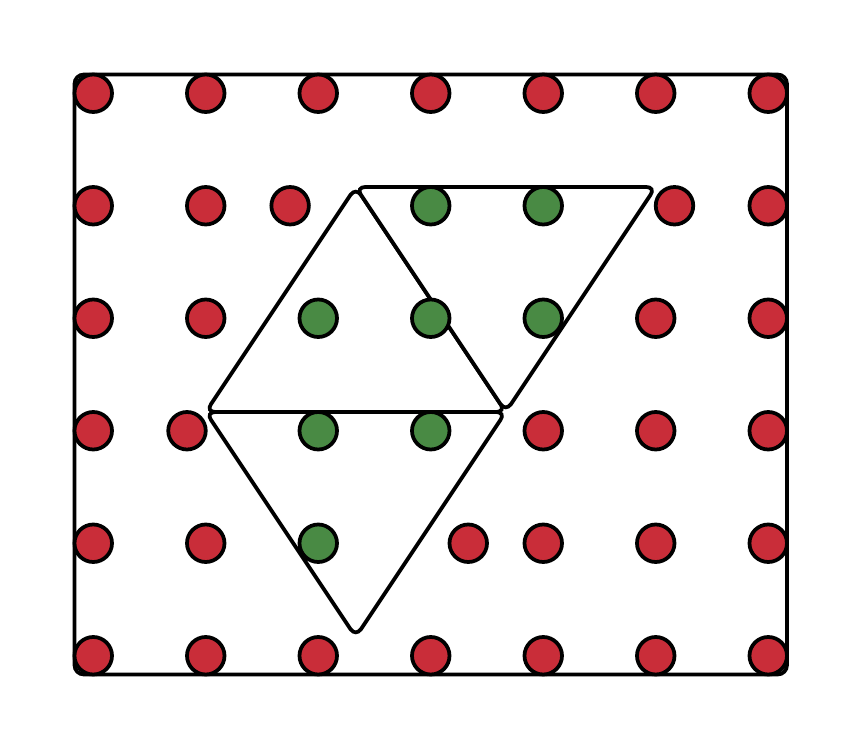
\includegraphics[width=0.9\textwidth]{bilder/m_points_inside}
     \caption{http://www.austincc.edu/rfofi/NursingRvw/PhysText/Cardiac.html}.
     \label{m_points_inside.png}
\end{figure}

\begin{figure}[h]
 \centering 
     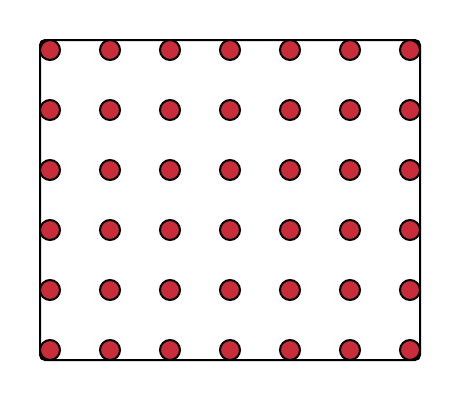
\includegraphics[width=0.9\textwidth]{bilder/m_grid_points}
     \caption{http://www.austincc.edu/rfofi/NursingRvw/PhysText/Cardiac.html}.
     \label{m_grid_points.png}
\end{figure}

\section{The Binary cube}




